% % LLNCS macro package for Springer Computer Science proceedings;
% Version 2.21 of 2022/01/12
%
\documentclass[runningheads]{llncs}
%
\usepackage[T1]{fontenc}
% T1 fonts will be used to generate the final print and online PDFs,
% so please use T1 fonts in your manuscript whenever possible.
% Other font encondings may result in incorrect characters.
%

\usepackage{amsmath}

\usepackage{graphicx, color, float, subfig}
\captionsetup{font=small,labelfont=bf,labelsep=period,skip=5pt}
\captionsetup[subfloat]{font=scriptsize,labelfont=bf,skip=5pt}

%
\usepackage{hyperref}
\renewcommand\UrlFont{\color{blue}\rmfamily}
\urlstyle{rm}
%

\begin{document}
\title{\fontsize{12}{12}\selectfont MAFIA: A Study of Subspace Clustering Algorithms}
\titlerunning{MAFIA: A Study of Subspace Clustering Algorithms}
%
\author{Henrik Daniel Christensen\orcidID{hench13@student.sdu.dk}}
\authorrunning{H. D. Christensen} % first names are abbreviated in the running head.
%
\institute{University of Southern Denmark, SDU\\\textit{Department of Mathematics and Computer Science}}
%
\maketitle % typeset the header of the contribution

%%%%%%%%%%%%%%%%%%%%%%%%%%%%%%%%%%%%%%%%%%%
\begin{abstract}
    This paper presents a comprehensive analysis of three bottom-up subspace clustering algorithms: \textit{MAFIA}, \textit{CLIQUE}, and \textit{SUBCLU}. MAFIA extends the grid-based approach of CLIQUE by introducing adaptive grid sizes, offering improved scalability and clustering quality. SUBCLU, in contrast, utilizes a density-connectivity method that allows better identification of arbitrarily shaped clusters, overcoming some of the limitations inherent in grid-based algorithms. The paper explores the relationships and distinctions between these algorithms, evaluating their performance in terms of scalability of dataset size, data- and cluster-dimensionality, as well as their clustering quality. Through a series of experiments with both synthetic and real-world datasets, we demonstrate the strengths and limitations of each approach. The findings reveal that while MAFIA is the most scalable, SUBCLU excels at detecting clusters with irregular shapes. However, all algorithms require proper parameter tuning for optimal performance.
    
    \keywords{High-Dimensional Subspace Clustering \and Grid-Based- and Density-Connectivity approach \and Comparative Study.}
\end{abstract}             % 0.4
\section{Introduction}
\textit{Clustering} is one of the main techniques within data mining. The main goal is to discover unknown patterns within a data set, by partitioning the data objects into \textit{clusters}. Here, each object in a cluster is similar to one another, but different from objects in other clusters. Clustering is widely used in many applications, such as advertising, biology, web search and business intelligence \cite[p.~444]{han-2011}.

The task of clustering data is a challenging task, first, the data sets are typical large in size, which means that the clustering algorithm must be \textit{scalable}. Additionally, data sets often contains numerous features (\textit{attributes}), which introduces the problem of \textit{curse of dimensionality}, which refers to a several challenges related to high-dimensional data spaces:

First, the issue of \textit{concentration of distances}, where distances between objects in high-dimensional spaces become increasingly similar as dimensionality increases. This means that data points tend to become nearly equidistant from one another, making it difficult for traditional distance-based algorithms to discover clusters.

Secondly, there is the problem of \textit{local feature relevance} and \textit{local feature correlation}, where only a subset of features or different combinations of feature correlations may be relevant for clustering. Consequently, feature reduction techniques like \textit{Principal Component Analysis} (PCA), which project the original space onto a lower-dimensional subspace, are inadequate because they typically identify only one global subspace that best fits the entire dataset. Also, algorithms that evaluate the entire feature space does not address this issue effectively. \cite[p.~43--46]{kriegel-2009}

Instead of relying on a global approach to feature selection, a local approach that addresses the issues of local feature relevance and local feature correlation is necessary. However, we then need to deal with two separate problems, which both needs to be solved simultaneously. First, is the problem of finding the relevant subspaces of each cluster. Second, is the problem of finding the clusters in each relevant subspace. To solve them efficiently, heuristics needs to be employed into the clustering algorithms. \cite[p.~6--7]{kriegel-2009}

For many applications, it is reasonable to focus only on clusters in axis-parallel subspaces, thus restricting the search space to $O(2^d)$ dimensions. These algorithms are called \textit{subspace clustering} (or \textit{projected clustering}) algorithms. These can be further divided into: \textit{top-down}- or \textit{bottom-up} approach. In top-down approach, the relevant subspaces for the clusters are determined by gradually reducing the subspaces, starting from the entire space. In contrast, bottom-up approaches, finds the relevant subspaces for the clusters from the original space starting from 1-dimensional using the \textit{monotonicity property} (or \textit{downward closure property}), see Lemma \ref{lem:mono} \cite{clique}. \cite[p.~8,~11]{kriegel-2009}

For the rest of this paper, the following notation will be adopted: Let $\mathcal{A} = \{A_1, \dots, A_d\}$ represent the set of dimensions (attributes) in a $d$-dimensional numerical space, $\mathcal{S} = A_1 \times A_2 \times \dots \times A_d$. A subset of $\mathcal{A}$ is called a subspace. Let $\mathcal{D} = \{p_1, \dots, p_n\}$ be the dataset, where $p_i \in \mathcal{S}$ represents a data point. A cluster $\mathcal{C}$ is a subset of $\mathcal{D}$, where each point $p_i \in \mathcal{C}$ is more similar to the other points in $\mathcal{C}$ than to points outside of $\mathcal{C}$.

\begin{lemma}\label{lem:mono}
    If $\mathcal{C}$ is a cluster in a $k$-dimensional subspace, then $\mathcal{C}$ must also form a cluster in any $(k-1)$-dimensional projection of the same space.
\end{lemma}
A proof is provided in \cite{clique}.

\subsection{Contributions}
The primary focus of this paper is to analyze the grid-based bottom-up subspace clustering algorithm \textit{MAFIA} \cite{mafia}, which builds upon the first grid-based approach \textit{CLIQUE} \cite{clique}. This paper examines the relationship between these two, highlighting their similarities and differences. Additionally, the density-connectivity-based algorithm \textit{SUBCLU} \cite{subclu} is included, as it offers a contrasting approach to the grid-based approach.

The remainder of the paper is structured as follows: Section 2 describes and analyzes the three algorithms in detail. Section 3 evaluates their performance in terms of scalability, considering dataset size, data- and cluster-dimensionality, as well as their clustering quality. Section 5 discusses the findings and explores the contributions of each algorithm to the field of subspace clustering. Finally, Section 6 concludes the main findings and suggests some future work.         % 1
\section{Subspace Clustering}
The main idea of subspace clustering is to identify subspaces of a high dimensional space to allow better clustering than the original (full) space. This is opposed to e.g. PCA, which projects the original space onto a new subspace, which may can be hard to interpret for the user.

Three different density-based subspace clustering algorithms will be discussed. First, the grid-based approach will be discussed, after which the density-based approach will be discussed. Note that, only bottom-up approaches will be considered in this paper.



\subsection{CLIQUE}
The key idea of grid-based subspace clustering is to partition the $\mathcal{S}$ into axis-parallel grid structure starting in 1-dimensional space. The grids forms hyper-rectangular \textit{units} (cells) for which we find the number of points in each. Only the units that exceeds a certain threshold are retained, called \textit{dense units}. Next, adjacent dense units will be merged to form so called \textit{candidate dense units} (CDUs), which will be used to find clusters in higher dimensional subspaces. The goal is then to describe the clusters using a minimal description in the form of DNF (\textit{Disjunctive Normal Form}) expressions.

CLIQUE is a bottom-up, grid-based subspace clustering algorithm that uses the monotonicity property as its clustering criterion, as described in Lemma \ref{lem:mono}.

The proof is provided in \cite{clique}.

The algorithm begins by partitioning the dataset $\mathcal{S}$ into equal-sized intervals (also called windows) of width $\varepsilon$ (input parameter), creating axis-parallel rectangular units. It then scans the dataset to identify 1-dimensional (1D) dense units by counting the number of points in each interval using a histogram, as shown in Figure \ref{fig:dense_cells_and_regions}. For example, with a grid size of $\varepsilon = 0.2$, three intervals in dimension $A_1$ exceed the density threshold $\tau$ (input parameter), while dimension $A_2$ reports four dense units. These dense units are known as \textit{candidate dense units} (CDUs).

The algorithm proceeds incrementally: it starts from 1D and moves to 2D, 3D, and so on, until no more CDUs can be generated. At each stage, the algorithm makes another pass over the dataset to determine which CDUs are dense in the higher dimensions, using the $(k-1)$-dimensional dense units identified in the previous stage. Specifically, CDUs in $k$ dimensions are formed by merging dense units in $(k-1)$ dimensions that share the first $(k-2)$ dimensions. This process continues until no further CDUs are generated.

To optimize performance, CLIQUE applies a pruning technique called \textit{coverage} (from \cite{clique}) to reduce computation time. This technique prunes subspaces with low coverage (i.e., those containing fewer points). However, this may risk eliminating subspaces that could potentially contain clusters.

Once all dense units are identified, CLIQUE defines clusters as maximal sets of connected dense units. For each $k$-dimensional subspace, the algorithm computes disjoint sets of connected dense units, where two units are connected if they share $k-1$ dimensions (a common face in the $k$-dimensional space) or if they are indirectly connected through other units. The algorithm then generates minimal cluster descriptions by covering each set of connected dense units with maximal regions and determining the minimal cover. For instance, in Figure \ref{fig:dense_cells_and_regions}, the minimal cover of the clusters is $A \cup B$, expressed as: $((0.2 \leq A_1 < 0.6) \land (0.4 \leq A_2 < 0.8)) \lor ((0.4 \leq A_1 < 0.8) \land (0.2 \leq A_2 < 0.6))$.
\begin{figure}[H]
    \vspace*{-0.5cm}
    \centering
    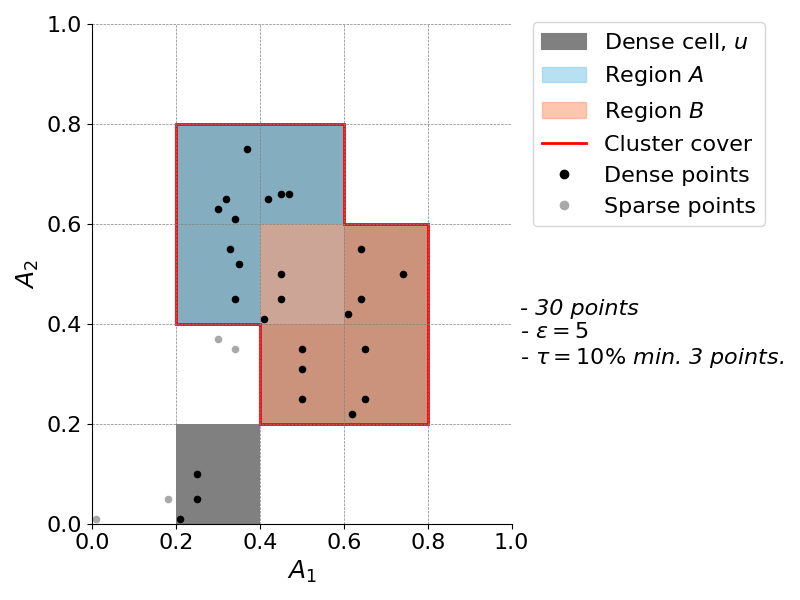
\includegraphics[width=0.4\textwidth]{figures/dense_cells_and_regions.png}
    \caption{Illustration of a dense unit $u$ and two overlapping dense regions $A$ and $B$.}
    \label{fig:dense_cells_and_regions}
    \vspace*{-0.5cm}
\end{figure}

\subsection{MAFIA}
MAFIA is an extension to CLIQUE where the grid sizes are adaptive meaning that the grid sizes are not fixed but are automatically determined by an algorithm. Moreover, the intention is not to rely on user specified input parameters like CLIQUE. In addition, MAFIA do not implement the pruning technique as noted in \cite{clique}, this could result in lost information.

The authors of MAFIA therefore introduces the \textit{Adaptive} algorithm, which starts by divide each dimension into a high number of equal-sized bins -- default it is $n = 1000$ bins. After dividing the dimension into $n$ bins, it merges the bins from left to right. Two bins are merged together if they are within a percentage of difference $\beta$ (input parameter). That means, a high beta value result in many merged bins, and vice-versa. If two bins are merged together, the highest bin count of the two are used to further merge with the next bin. An example is shown in Figure \ref{fig:adaptive_grids}, where in (a) shows the bins before merging and in (b) shows the bins after merging. The result of the algorithm, as can be seen in the figure, is that bins with similar counts are merged together. At last the algorithm determines a so called \textit{threshold-level} for each of the variable-sized bins. The threshold-level is determined by the size of the bin and a so called \textit{cluster dominance factor} $\alpha$ (input parameter). A higher $\alpha$ will result in a higher threshold-level, meaning that the bin must contain more points to be considered a dense unit, and vice-versa.

\begin{figure}[H]
    \vspace*{-0.5cm}
    \centering
    \subfloat[][Uncombined bins]{%
        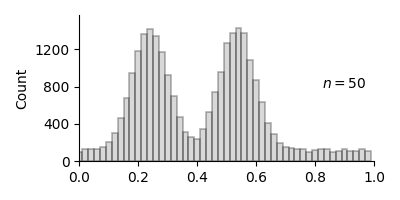
\includegraphics[width=0.4\textwidth]{figures/uncombined_histogram.png}\label{fig:uncombined_bins}}~~~~
    \subfloat[][Combineed bins]{%
        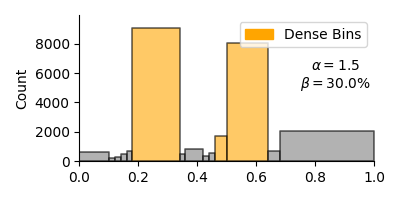
\includegraphics[width=0.4\textwidth]{figures/combined_histogram.png}\label{fig:combined_bins}}~~~~
    \caption{Illustration of the adaptive grids computation.}
    \label{fig:adaptive_grids}
    \vspace*{-0.5cm}
\end{figure}

Having completed the adaptive grid computation, MAFIA proceeds like CLIQUE by scanning the dataset to identify dense units in each subspace. However, the CDUs are generated differently.

\subsubsection{CDU Generation}

\subsection{SUBCLU}
A drawback of grid-based methods is that the quality of clustering depends on the positiong of the grids. In Figure \ref{fig:dense_cells_and_regions}, we see that the due to the rigid grid structure we might miss cluster points, that is point not in a dense cell. This problem especially occurs for clusters that are not of rectangular shapes. In contrast, SUBCLU which extends the principles of DBSCAN to subspaces, that is it relies on the locality assumption of points.

The algorithm starts by identifying clusters in 1-dimensional subspaces, applying DBSCAN to each attribute separately. In this step, it looks for dense regions using a parameter $\epsilon$, which defines the radius within which points are considered neighbors, and $m$, the minimum number of points required for a region to be dense. If clusters are detected in these 1-dimensional subspaces, they are further explored in higher dimensions.

The next phase involves a bottom-up approach where the algorithm combines previously detected $k$-dimensional subspaces that share $k-1$ attributes to generate $(k+1)$-dimensional candidate subspaces. By extending the clusters found in lower-dimensional subspaces, SUBCLU tests if they persist when new dimensions are added. DBSCAN is again applied in these candidate subspaces with the same $\epsilon$ and $m$ values, checking whether clusters detected in the lower-dimensional space still qualify as clusters when higher dimensions are included.

Efficiency is achieved through the monotonicity property of density-connected sets: if no clusters exist in a $k$-dimensional subspace, then higher-dimensional subspaces derived from it will not contain clusters, allowing the algorithm to prune the search space.

For candidate subspaces where clusters are found, SUBCLU further refines these clusters by choosing subspaces with minimal numbers of objects in the clusters, which reduces the computational load when expanding them into higher dimensions.  % 2
\section{Evaluation}
The evaluation of the clustering algorithms was performed on a Intel i7 1.70 GHz processor (12th gen.) with 16 GB of RAM running Windows 11.

The evaluation of MAFIA was performed using \textit{GPUMAFIA} \cite{gpumafia}, which was installed on a virtual machine (VM) running Ubuntu. The VM was configured with 4 CPUs and 4 GB of RAM.

CLIQUE and SUBCLU were evaluated on the main machine using \textit{ELKI} \cite{elki}. Thus, one should be careful to compare the results of the three algorithms directly, as the execution environment and the implementation may affect the results. However, the growth rate and their clustering of the data sets can be compared.

Throughout the different experiments, a range of input parameters for the three algorithms were tested. The best found were selected. The complete evaluation project can be found in the GitHub repository: \url{https://github.com/henrikdchristensen/SDU-Data-Mining-Exam}. Here, additional experiments as well as detailed descriptions of how to generate the data sets and how to install and use GPUMAFIA is described.

\subsection{Data set generation}
The aim for the synthetic data generation was to be able to produce similar data sets as discussed in \cite{clique,mafia}. That is, hyper-rectangles (axis-parallel) clusters in different subspaces. This was achieved by using \textit{MDCGen}, where different sizes and different densities of the clusters could be determined, as well as which attributes for each cluster that are noise for which values at random is selected from a uniform distribution over the entire range of the attribute.

However, to see the one of the main advantages of SUBCLU compared to CLIQUE and MAFIA, a data set containing a Bezier-shaped cluster was created using \textit{Artificial Cluster} (AC). In addition, a self-populated data set containing a plus-shaped cluster was created as discussed in \cite{mafia}.

Finally, two real-world data sets were selected to evaluate the algorithms in a more realistic setting.

All the data sets were normalized such that each attribute was in the range [0, 1].

\subsection{Experimental Results}

\subsubsection{Scalability with Data Set Size}
To evaluate the scalability of the algorithms a data set containing 20 dimensions with 5 clusters in 5 different subspaces with 10\% noise records was used. The data set size ranges from 10k to 1mio records. The results can be seen in Figure \ref{fig:dataset_size_vs_runtime}. As can be seen, MAFIA is the most scalable algorithm of the three. CLIQUE could handle up to 500k records, while SUBCLU was only able to handle up to 100k records. Similar results in terms of growth rate were reported in all three papers \cite{mafia,clique,subclu}. That is, linear growth for MAFIA and CLIQUE, and quadratic growth for SUBCLU. The linear behaviour of CLIQUE and MAFIA comes from the fact that the number of passes over the data set depends only on the dimensionality of the embedded cluster. An increase in the size of the data set just means that more data has to be scanned on every pass over the data set while finding dense units resulting in a linear growth rate. SUBCLU, on the other hand, has a quadratic growth rate, as it relies on the DBSCAN algorithm which needs partial range queries that can be costly in terms of running time. Better running time of all three is achieved compared to the three papers. This is probably, due to better hardware.

Note that, the \texttt{minpts} in SUBCLU were scaled linearly with the data set size, as the clusters in the dateset were of a fixed size, which means, by increasing the data set size, the density of the clusters increases linearly. However, for the other two algorithms, there was no need to scale any of input parameters, as they relies on the density of the units for the total amount of records.
\begin{figure}[H]
    \vspace*{-0.5cm}
    \centering
    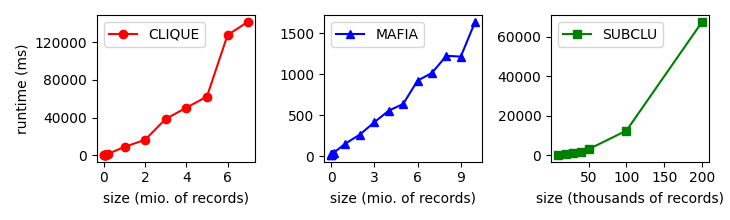
\includegraphics[scale=0.45]{figures/dataset_size_vs_runtime.png}
    \caption{Scalability with increasing data set size.}
    \label{fig:dataset_size_vs_runtime}
    \vspace*{-0.5cm}
\end{figure}

\subsubsection{Clustering Accuracy}
Many different synthetic data sets were generated to test the clustering accuracy of the algorithms.

The first data set were a 2-dimensional data set containing a single cluster formed as a skewed plus-sign with 10\% noise added. Similarly results as in \cite{mafia} was achieved, MAFIA detects the 2-dimensional cluster accurately, whereas CLIQUE finds two overlapping clusters, where none of these detects the borders correctly. The accuracy of MAFIA comes, however, with a cost, as it also reports some lower-dimensional clusters as well.
% The results can be seen in Figure \ref{fig:accuracy_plus}, where only the best cluster found by MAFIA is illustrated. The effect of adaptive grid sizes, clearly shows that MAFIA is more flexible than CLIQUE in such cases.
% \begin{figure}[H]
%     \vspace*{-0.5cm}
%     \centering
%     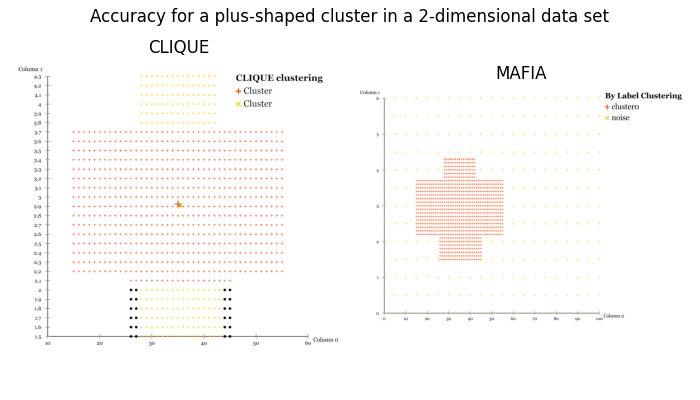
\includegraphics[scale=0.35]{figures/accuracy_plus.png}
%     \caption{A single plus-shaped cluster.}
%     \label{fig:accuracy_plus}
%     \vspace*{-0.5cm}
% \end{figure}

The second data set contains 10 dimensions with contains 2 clusters embedded in a different 4 dimensional subspace. 10\% of the data was added as noise records. Similar data set as the one used in \cite{mafia}. The results can be seen in Figure \ref{fig:accuracy_2clusters}. Here, MAFIA was able to detect the clusters without any additional lower-dimensional clusters. In contrast, CLIQUE reports some overlapping clusters and some of the noise records as clusters. SUBCLU detects also the two clusters, but reports many lower-dimensional clusters and noise records as clusters as well.
\begin{figure}[H]
    \vspace*{-0.5cm}
    \centering
    \subfloat[][CLIQUE]{%
        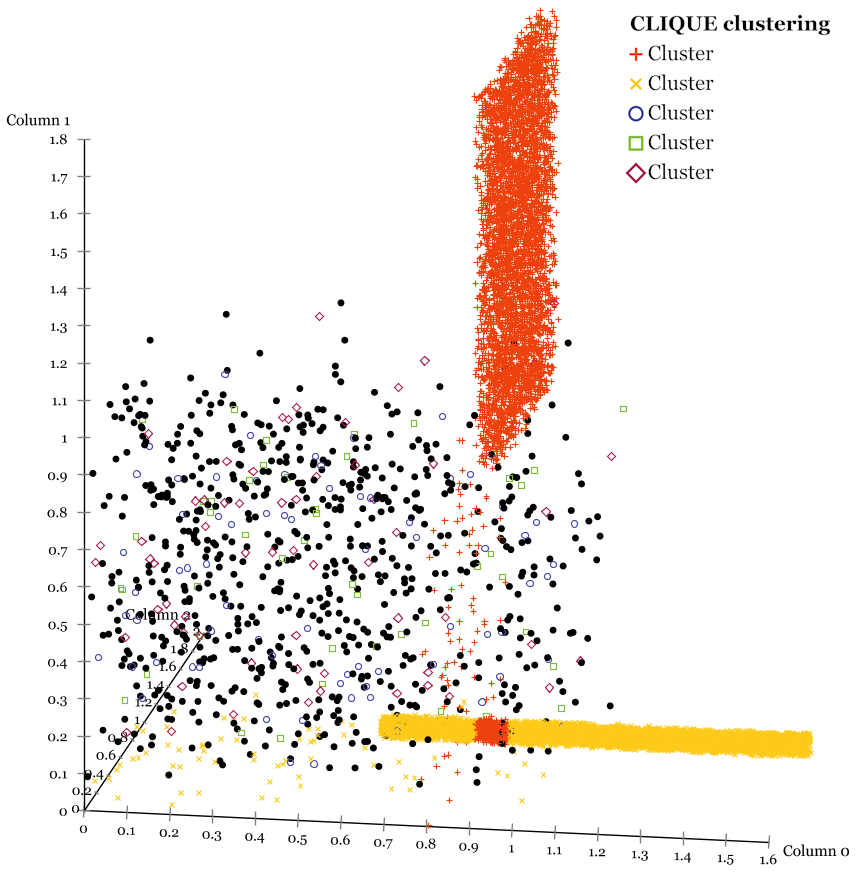
\includegraphics[width=0.3\textwidth]{figures/accuracy_2clusters/clique.png}\label{fig:accuracy_2clusters_clique}}~~~~
    \subfloat[][MAFIA]{%
        \includegraphics[width=0.3\textwidth]{figures/accuracy_2clusters/MAFIA.png}\label{fig:accuracy_2clusters_mafia}}~~~~
    \subfloat[][SUBCLU]{%
        \includegraphics[width=0.3\textwidth]{figures/accuracy_2clusters/SUBCLU.png}\label{fig:accuracy_2clusters_subclu}}
    \caption{Two clusters in 4 different subspaces.}
    \label{fig:accuracy_2clusters}
    \vspace*{-0.5cm}
\end{figure}

The third data set were a 2-dimensional data set containing a single cluster formed as a Bezier curve with 10\% noise added to the data set. As expected, SUBCLU outperforms the other two algorithms as can be seen in Figure \ref{fig:accuracy_bezier}. MAFIA and CLIQUE only partly detects the cluster and reports additional clusters and noise records as clusters. The result of SUBCLU demonstrates its locality assumption and its use of DBSCAN.
\begin{figure}[H]
    \vspace*{-0.5cm}
    \centering
    \subfloat[][CLIQUE]{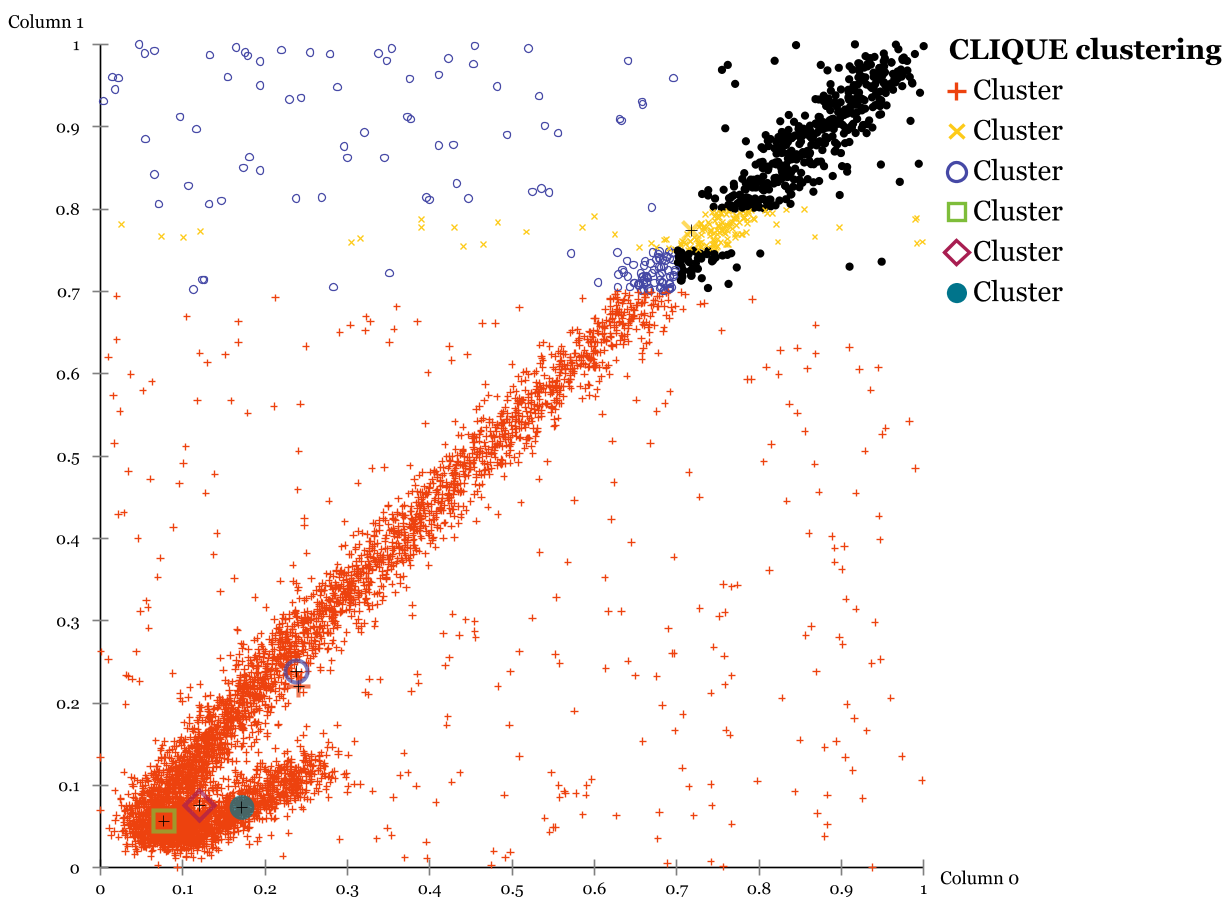
\includegraphics[width=0.3\textwidth]{figures/accuracy_bezier/clique.png}\label{fig:accuracy_bezier_clique}}~~~~
    \subfloat[][MAFIA]{\includegraphics[width=0.3\textwidth]{figures/accuracy_bezier/MAFIA.png}\label{fig:accuracy_bezier_mafia}}~~~~
    \subfloat[][SUBCLU]{\includegraphics[width=0.3\textwidth]{figures/accuracy_bezier/SUBCLU.png}\label{fig:accuracy_bezier_subclu}}
    \caption{A single bezier-shaped cluster.}
    \label{fig:accuracy_bezier}
\end{figure}

\subsubsection{Scalability with Data Dimensionality and Cluster Dimensionality}
Figure \ref{fig:data_dimensionality_vs_runtime} shows the scalability of the CLIQUE and MAFIA with increasing data set dimensionality. The data set contains 1 mio. records with 3 clusters in 5 different subspaces and 10\% noise records, similar to the data set in \cite{mafia}. The data set dimensionality ranges from 10 to 100 dimensions. However, CLIQUE was only able to handle half of the dimensions, as the PC constantly freezes -- probably due to the high memory consumption. In \cite{clique} it is noted that CLIQUE has a quadratic growth rate in terms of data set dimensionality. To investigate this even further, one could try to reduce the memory consumption by having a smaller amount of records in the data set. Nevertheless, MAFIA is the most scalable algorithm of the two.
\begin{figure}[H]
    \vspace*{-0.5cm}
    \centering
    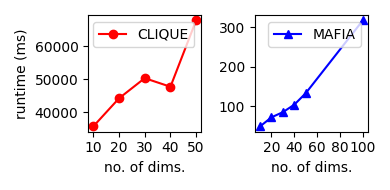
\includegraphics[scale=0.45]{figures/data_dimensionality_vs_runtime.png}
    \caption{Scalability with increasing data set dimensionality.}
    \label{fig:data_dimensionality_vs_runtime}
    \vspace*{-0.5cm}
\end{figure}

Figure \ref{fig:cluster_dimensionality_vs_runtime} shows the scalability of the CLIQUE and MAFIA with increasing cluster dimensionality. A 20-dimensional data set, containing 500k records with a single cluster were used. The cluster was embedded in increasing number of dimensions starting from 10 to 100 dimensions. 10\% of the records was added as noise. The data set is similar to the one used in \cite{mafia}. Both algorithms heavily suffers from the increasing cluster dimensionality, however, MAFIA is able to handle a higher dimensional cluster than CLIQUE. The reason why both algorithms depends on the cluster dimensionality is due to the fact that a higher cluster dimensionality results in a large subspace coverage and a large number of CDUs. In other words, each pass on the data needs to populate a large number of CDUs, adn increase in cluster dimensionality also increases the number of passes over the data set.
\begin{figure}[H]
    \vspace*{-0.5cm}
    \centering
    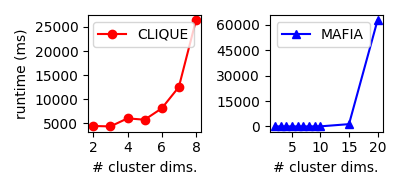
\includegraphics[scale=0.45]{figures/cluster_dimensionality_vs_runtime.png}
    \caption{Scalability with increasing cluster dimensionality.}
    \label{fig:cluster_dimensionality_vs_runtime}
    \vspace*{-0.5cm}
\end{figure}

The results reported for SUBCLU in \cite{subclu} were also tried to be replicated, however, similar it was not possible evaluate in different scales of data set dimensionality and cluster dimensionality, as the PC constantly freezes -- probably due to the high memory consumption. In future work, it would be interesting to investigate this further.

% \subsection{Sensitive analysis for MAFIA}
% From \cite{mafia}, MAFIA should not be sensitive to the choice of $\alpha$. Therefore, a 20-dimensional data set with 1mio data points with 10\% noise were set to evaluate this. $\beta$ was fixed to 35\%, and $\alpha$ was ranging from 0.8 to 5.2 in step size of 0.4. The results can be seen in Figure \ref{fig:sensitivity_alpha}. From the results one could again draw the conclusion that MAFIA is not very sensitive to the $\alpha$ parameter. However, during evaluation of different types of data sets, many different values $\alpha$ was used to detect the right clusters. Also, different $\beta$ values as well as maximum number of windows was needed to be set properly to achieve meaningful results.
% \begin{figure}[H]
%     \vspace*{-0.5cm}
%     \centering
%     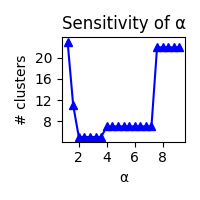
\includegraphics[scale=0.45]{figures/sensitivity_alpha.png}
%     \caption{Sensitivity of $\alpha$ for MAFIA.}
%     \label{fig:sensitivity_alpha}
% \end{figure}

\subsubsection{Real Data Sets}
Two real-world data sets are used to evaluate the algorithms in a more realistic setting. Small data sets were selected for both performance and visualization reasons. Both data sets were normalized such that each attribute was in the range [0, 1].

The first data set is the well-known \textit{Iris} data set \cite{iris}, which contains 150 records of 3 different iris types (e.g. Setosa, Versicolor, Virginica). The data set contains 4 features (sepal length, sepal width, petal length and petal width). All three algorithms produced some meaningful clusters, however, as can be seen in Figure \ref{fig:real_world_iris}. It is hard to determine which algorithm performs the best in this case.
\begin{figure}[H]
    \vspace*{-0.5cm}
    \centering
    \subfloat[][Original]{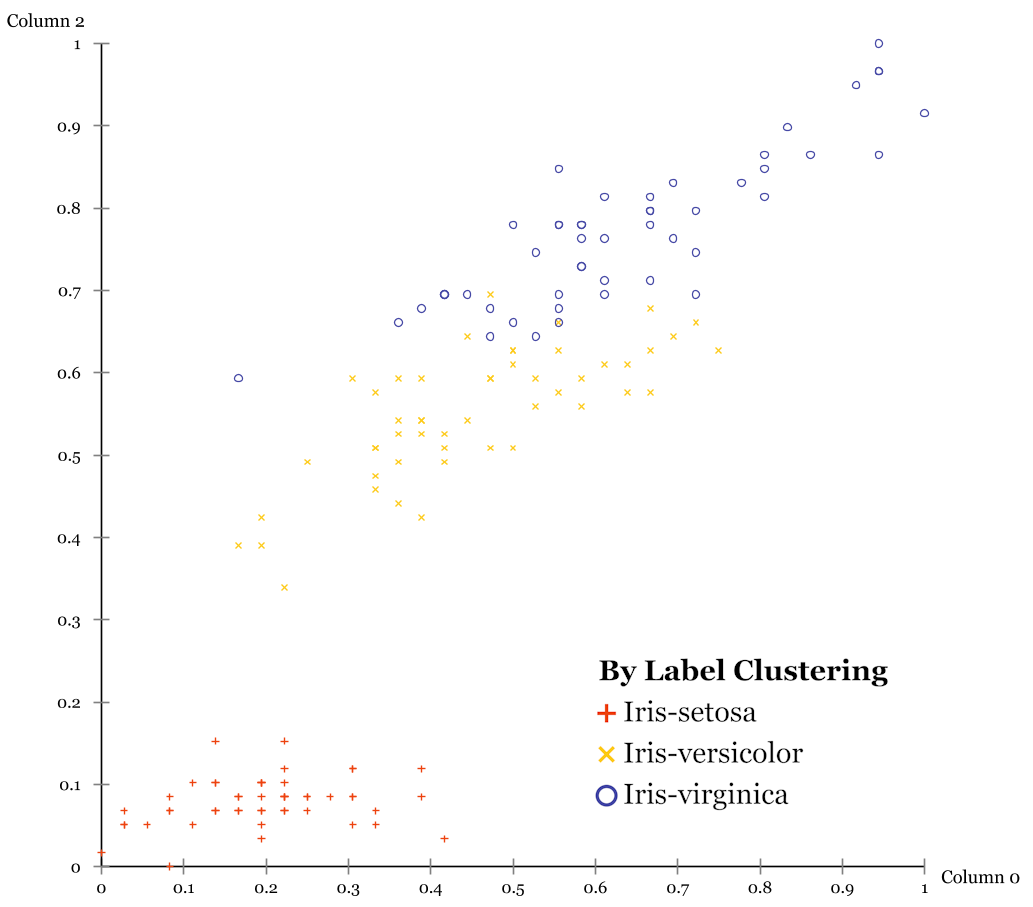
\includegraphics[width=0.3\textwidth]{figures/real_world_iris/orig.png}\label{fig:real_world_iris_orig}}~~~~
    \subfloat[][CLIQUE]{\includegraphics[width=0.3\textwidth]{figures/real_world_iris/CLIQUE.png}\label{fig:real_world_iris_clique}}\\
    \subfloat[][MAFIA]{\includegraphics[width=0.3\textwidth]{figures/real_world_iris/MAFIA.png}\label{fig:real_world_iris_mafia}}~~~~
    \subfloat[][SUBCLU]{\includegraphics[width=0.3\textwidth]{figures/real_world_iris/SUBCLU.png}\label{fig:real_world_iris_subclu}}
    \caption{Iris data set.}
    \label{fig:real_world_iris}
    \vspace*{-0.5cm}
\end{figure}

The second data set is the \textit{Date Fruit} data set \cite{date-fruit}, which contains 898 records of 7 different date fruit types (e.g. Barhee, Deglet Nour, Sukkary, Rotab). These were obtained via a computer vision, where 34 features (e.g shape and color) was extracted. Only SUBCLU were able to produce clusters somewhat close to the true clusters but also finds many lower-dimensional clusters and small clusters. CLIQUE and MAFIA either produced way too many clusters or close to one single cluster.
% \begin{figure}[H]
%     \vspace*{-0.5cm}
%     \centering
%     \subfloat[][Original]{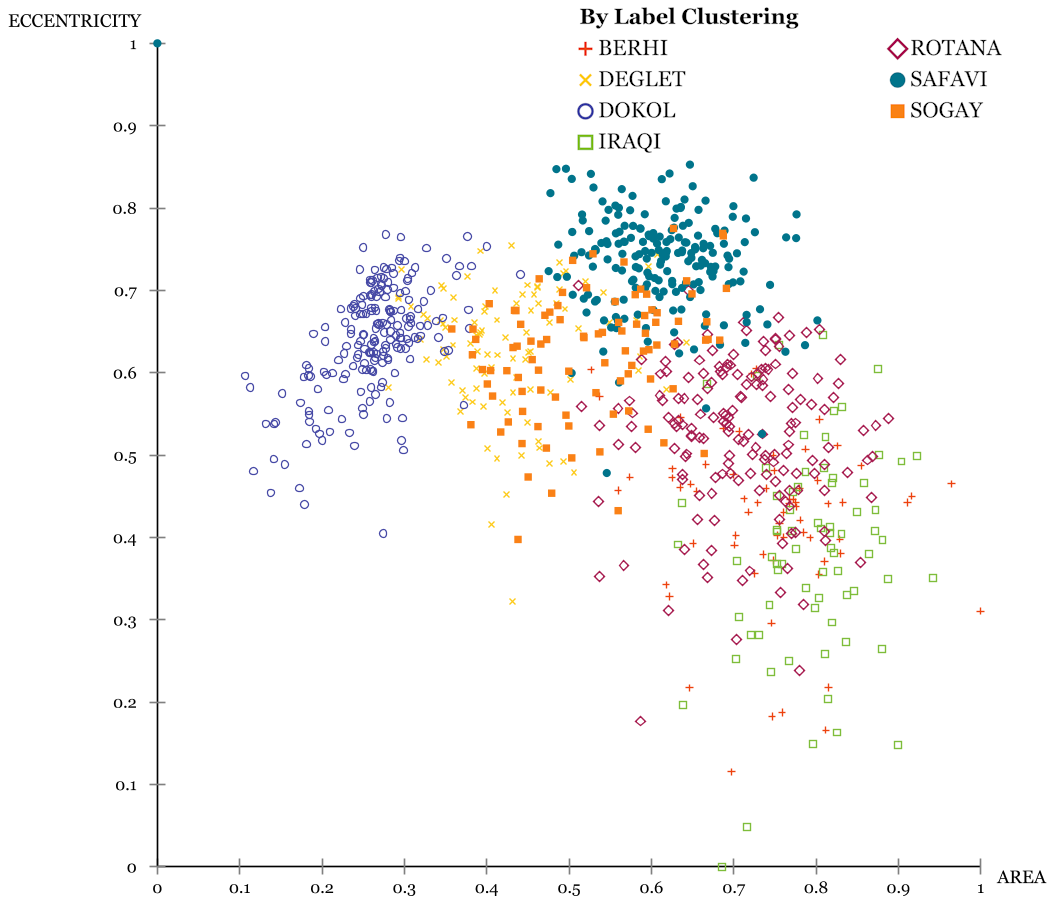
\includegraphics[width=0.3\textwidth]{figures/real_world_date_fruit/orig.png}\label{fig:real_world_date_fruit_orig}}~~~~
%     \subfloat[][SUBCLU]{\includegraphics[width=0.3\textwidth]{figures/real_world_date_fruit/SUBCLU.png}\label{fig:real_world_date_fruit_subclu}}
%     \caption{Date Fruit data set.}
%     \label{fig:real_world_date_fruit}
% \end{figure}           % 3
\section{Discussion}
CLIQUE, MAFIA, and SUBCLU are three prominent subspace clustering algorithms, each offering unique strengths and limitations. CLIQUE, as one of the earliest subspace clustering approaches, uses a grid-based method where the data space is partitioned into equi-sized cells, and dense units are identified based on a density threshold. The advantage of CLIQUE is its simplicity and efficiency in navigating through subspaces using an Apriori-like strategy. However, its reliance on fixed grid boundaries can lead to issues when clusters do not align with these grids, resulting in missed or fragmented clusters. Moreover, the algorithm is sensitive to grid size and density thresholds, which may not be optimal for all datasets.

MAFIA builds upon CLIQUE by introducing adaptive grid sizes, allowing it to dynamically adjust grid boundaries based on data density. This modification enables MAFIA to detect clusters more precisely, providing better resolution than CLIQUE, especially in complex datasets. Additionally, experiments indicate that MAFIA is the most scalable algorithm when it comes to handling large data sizes. However, this scalability comes at a cost; MAFIA is highly sensitive to input parameters, such as grid size and density thresholds, and requires careful tuning to achieve optimal results. While it offers more precise boundary detection than CLIQUE, its dependence on parameters can lead to inconsistent performance across different datasets.

SUBCLU, on the other hand, departs from the grid-based approach and utilizes a density-connectivity principle similar to DBSCAN. This enables it to detect clusters of arbitrary shapes, which is a significant advantage when clusters are irregular or not aligned with the axes. This was demonstrated in experiments using real datasets, where SUBCLU outperformed grid-based methods in identifying clusters with complex boundaries. However, SUBCLU’s approach, while flexible, may not be as efficient as MAFIA in terms of data size scalability, particularly for very large datasets.

A critical observation across these algorithms is that their performance can vary significantly depending on the data characteristics. Experiments using synthetic data show that clustering quality is highly use-case dependent, and allowing or disallowing lower-dimensional clusters can affect outcomes. Furthermore, while these synthetic experiments highlight each algorithm’s strengths, they also reveal their limitations. It is possible to generate datasets where none of these methods can identify the correct clusters, showing that subspace clustering remains a challenging problem.

All three algorithms struggle with closely clustered data points, often requiring fine-tuning of parameters such as grid size in CLIQUE and MAFIA, or \( \epsilon \) and \( m \) in SUBCLU, to effectively separate clusters. This need for parameter optimization underscores the complexity of subspace clustering and the necessity for tailored solutions depending on the specific data distribution and clustering objectives.           % 3
\section{Conclusion}
In conclusion, this study highlighted the strengths and limitations of three subspace clustering algorithms, with a particular focus on MAFIA. MAFIA's adaptive grid approach has proven to be the most scalable, making it ideal for large datasets where computational efficiency is paramount. Its flexibility in adapting to the data structure allows for better performance, but this comes with the challenge of more complex parameter tuning. CLIQUE, while also scalable, suffers from reduced clustering quality in more complex data distributions due to its reliance on fixed grid sizes. SUBCLU, with its density-connected method, excels at detecting arbitrarily shaped clusters, but its higher computational cost limits its scalability. MAFIA's ability to balance scalability and clustering quality, particularly in large-scale data sets, ,makes its a powerful tool in subspace clustering. However, future work could further refine MAFIA's parameter sensitivity.           % 0.5
%%%%%%%%%%%%%%%%%%%%%%%%%%%%%%%%%%%%%%%%%%%

%%%%%%%%%%%%%%%%%%%%%%%%%%%%%%%%%%%%%%%%%%%
%\begin{credits}
    \subsubsection{\ackname}
    A bold run-in heading in small font size at the end of the paper is
    used for general acknowledgments, for example: This study was funded
    by X (grant number Y).
    
    \subsubsection{\discintname}
    It is now necessary to declare any competing interests or to specifically
    state that the authors have no competing interests. Please place the
    statement with a bold run-in heading in small font size beneath the
    (optional) acknowledgments\footnote{If EquinOCS, our proceedings submission
    system, is used, then the disclaimer can be provided directly in the system.},
    for example: The authors have no competing interests to declare that are
    relevant to the content of this article. Or: Author A has received research
    grants from Company W. Author B has received a speaker honorarium from
    Company X and owns stock in Company Y. Author C is a member of committee Z.
\end{credits}


\bibliographystyle{base/splncs04}
\bibliography{base/references}
%%%%%%%%%%%%%%%%%%%%%%%%%%%%%%%%%%%%%%%%%%%
\end{document}